\documentclass{beamer}
\usepackage{beamerthemesplit}
\usepackage{amsmath}
\usepackage{adjustbox}
\usepackage{amssymb}
\usepackage{subfigure}
\usepackage{amsfonts}
\usepackage{newlfont}
\usepackage{graphics}
\usepackage{graphicx}
\usepackage{epsfig}
\usepackage{booktabs}
\usepackage{booktabs, longtable,array}


\usepackage[english]{babel}
\usepackage[latin1]{inputenc}
%\usepackage{hyperref}
%\usepackage[round]{natbib}

% \usetheme{default}
% \usetheme{Boadilla} %# not so good
% \usetheme{Madrid}  % # not so good
% \usetheme{Montpellier}
% \usetheme{Warsaw}
% \usetheme{Copenhagen}
% \usetheme{Goettingen}
% \usetheme{Hannover}
%\usetheme{Berkeley}
\usecolortheme{orchid}
\beamertemplatesolidbackgroundcolor{white!65}
\setlength{\parskip}{8pt plus 1pt minus 1pt}
\setbeamertemplate{footline}[frame number]


\title[]{LOW COST HARDWARE DESIGN FOR IoT
APPLICATION IN INDUSTRIAL PROCESS}
\author{B.Tech Project Presentation Group Number-07}
\author{Gundappa DH (2015IPG-032)\\
        Kuthadi Sanjeev Kumar (2015IPG-046)\\
        Sachin Nikunj (2015IPG-78)\\
\vspace{6mm}
\textbf{Supervised by: Dr. Prasenjit Chanak}} 

\institute[]{
	
	ABV-Indian Institute of Information Technology and\\
	Management, Gwalior
}
\date{\today}


\begin{document}
	\frame{\titlepage}
	
	%\begin{frame}
	%\frametitle{Outline}
	%\tableofcontents[pausesections]
	%\end{frame}
	
	\begin{frame}\frametitle{Contents}
	\begin{itemize}
		\item	Introduction
		\item   literature review 
		\item   Objective 
		\item	Proposed scheme
		\item   Testing
		\item	Results
		\item   Conclusion and Future works
		\item   References
	\end{itemize}
\end{frame}
\begin{frame}\frametitle{Introduction}
\begin{itemize}
\item Internet Of Things
\begin{itemize}
	\item Is a network of physical objects, embedded with sensors, electronics and soft wares.	 
	\item Which enables network connectivity and helps in collecting and exchanging the data.	  
\end{itemize}
\item Importance
\begin{itemize}
\item It can be next industrial revolution in terms of automation. 
\item Makes easy to integrate all the objects for making the devices.
\end{itemize}
\end{itemize}
\end{frame}
\begin{frame}[shrink=20]\frametitle{Literature review}
\begin{table}[h]
    \begin{tabular}{|c|p{3cm}|p{3cm}|p{3cm}|}
    \hline
    \textbf{S.No} & \textbf{Paper Title} & \textbf{Authors} & \textbf{Details and Limitations}\\
    \hline 
    1 &Applications for ultrasonic sensors in process industries &  Puttmer, Alf &Application of ultrasonic sensor in automation and changing the labour engagement.\\
    \hline
    2 &Raspberry Pi as Internet of things hardware: performances and constraint & Maksimovic, Mirjana, et al & Major application of Raspberry pi in industrial process and its importance in automation sector.\\
    \hline
    3 & A novel ultrasonic sensing system for autonomation  &  Bank, Dirk & Major application in decreasing employee engagement by using it in a health monitoring system.\\
    \hline
 
  \end{tabular}
  %\caption{This table shows some data}
  %\label{tab:myfirsttable}
\end{table}
\end{frame}

\begin{frame}\frametitle{Objective}
\begin{itemize}

\item To design a multi sensor based device for data acquisition.
\item Connect different multi sensor based data acquisition board through an energy efficient communication scheme.
\item To design data acquisitions scheme to collect real life data from different deployed multi sensor based data acquisition board.
\item To design a scheme to analyze the collected data for identification of fault of the industrial machine Transmission of data to cloud platform.

\end{itemize}
\end{frame}
\begin{frame}\frametitle{Proposed scheme}

\begin{itemize}
	\item Our proposed scheme mainly work in industrial sector, to identify the machines health condition .	 
	\item When ever machines gets damaged it becomes really hard to identify the problem early but we can find some changes in sound, vibration, smoke, temperature of the machines .	 
	\item At some of the places where machines work there we humans cannot observe its working, some sensors can be used instead of humans and it becomes cost efficient for the companies. 
\end{itemize}

\end{frame}
\begin{frame}\frametitle{Proposed scheme}

\begin{itemize}
\begin{figure}[h]
\centerline{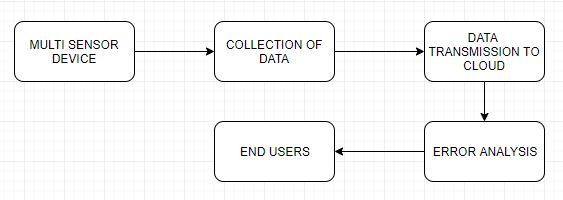
\includegraphics[width=3.7in]{SCHEME}}
\caption{Proposed schematic diagram .}
\end{figure}
	\item As the above picture depicts the scheme, we collect the data from the multiple sensor.	 
	\item Collected data gets transmitted into cloud using the wi-fi sensor.	 
	\item  hen we get the data in cloud platform we identify the variations in data, which we receive from the multi sensors device.
\end{itemize}

\end{frame}

\begin{frame}\frametitle{Implementation}
\item Major implementations of our objective 
\begin{itemize}

\item Integration of ultrasonic sensor and sound sensor on a micro controller.
\item Integration of Multiple sensors on a micro controller.
\item Communication of data between two devices.
\item Transmission of data to cloud platform.

\end{itemize}
\end{frame}
\begin{frame}\frametitle{Integration of ultrasonic senor and sound sensor on a micro controller}
\begin{itemize}
\item We have used ultrasonic sensor to calculate the distance of the object placed in front of the sensor.
\item The sound sensor is used to calculate the  sound variations in the  surroundings
\end{itemize}
\end{frame}
\begin{frame}\frametitle{Architecture of Basic master device}
\begin{itemize}
  \begin{figure}[H]
  \centerline{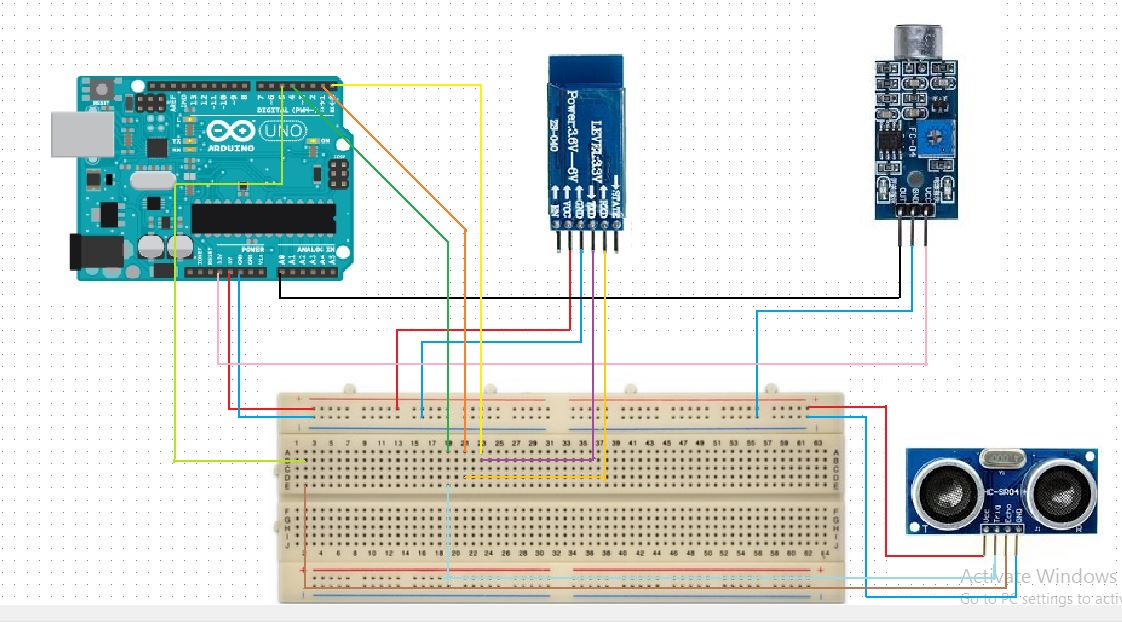
\includegraphics[width=4.0in]{master.JPG}}
  \caption{ \textbf{}Master device architecture}
  \end{figure}
\end{itemize}
\end{frame}
\begin{frame}[shrink=10]\frametitle{Architecture of basic slave device }
\begin{itemize}
\begin{figure}[h]
\centerline{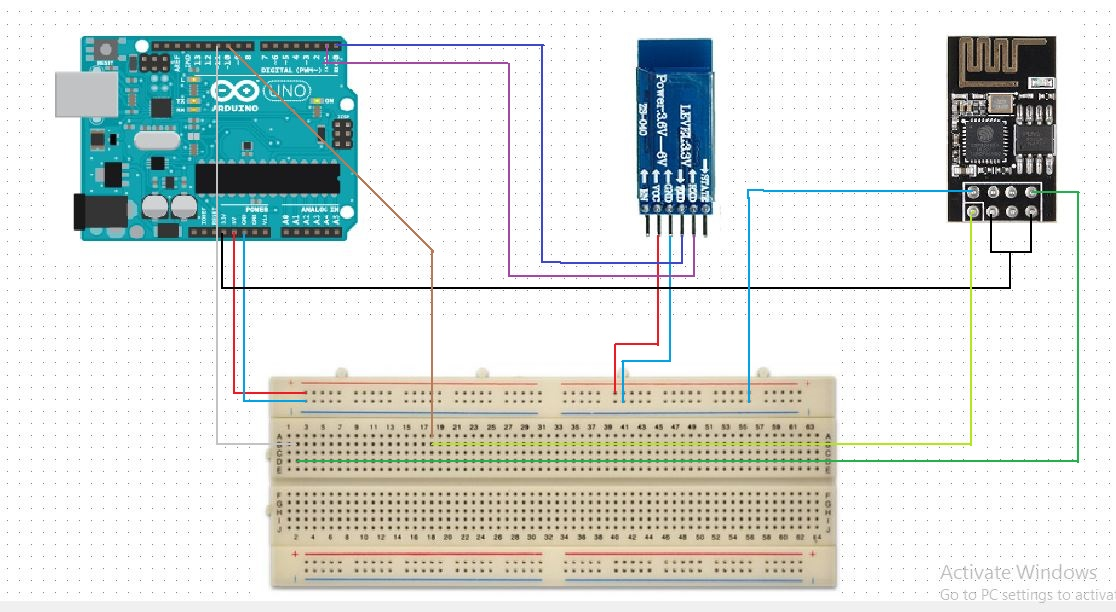
\includegraphics[width=3.7in]{slave}}
\caption{slave device architecture  .}
\end{figure}
\end{itemize}
\end{frame}
  \begin{frame}\frametitle{Integration of multiple sensors on a micro controller}
 \item Smoke  sensor
\begin{itemize}
\item Smoke sensor is used to detect a wide range of gases in the surroundings.
\item Wide range of gases include propane, butane, hydrogen etc.
\end{itemize}
 \item Vibration sensor
\begin{itemize}
    \item Vibration sensor is used to feel the vibration in the surroundings. 
    \end{itemize}
    \item Humidity and Temperature sensor
    \begin{itemize}
        \item Humidity and temperature sensor is used to calculate the relative humidity in the air
        \item It is also used to calculate the change in the temperature in the surroundings.
    \end{itemize}
\end{frame}

\begin{frame}\frametitle{Master device}
  \begin{figure}[H]
  \centerline{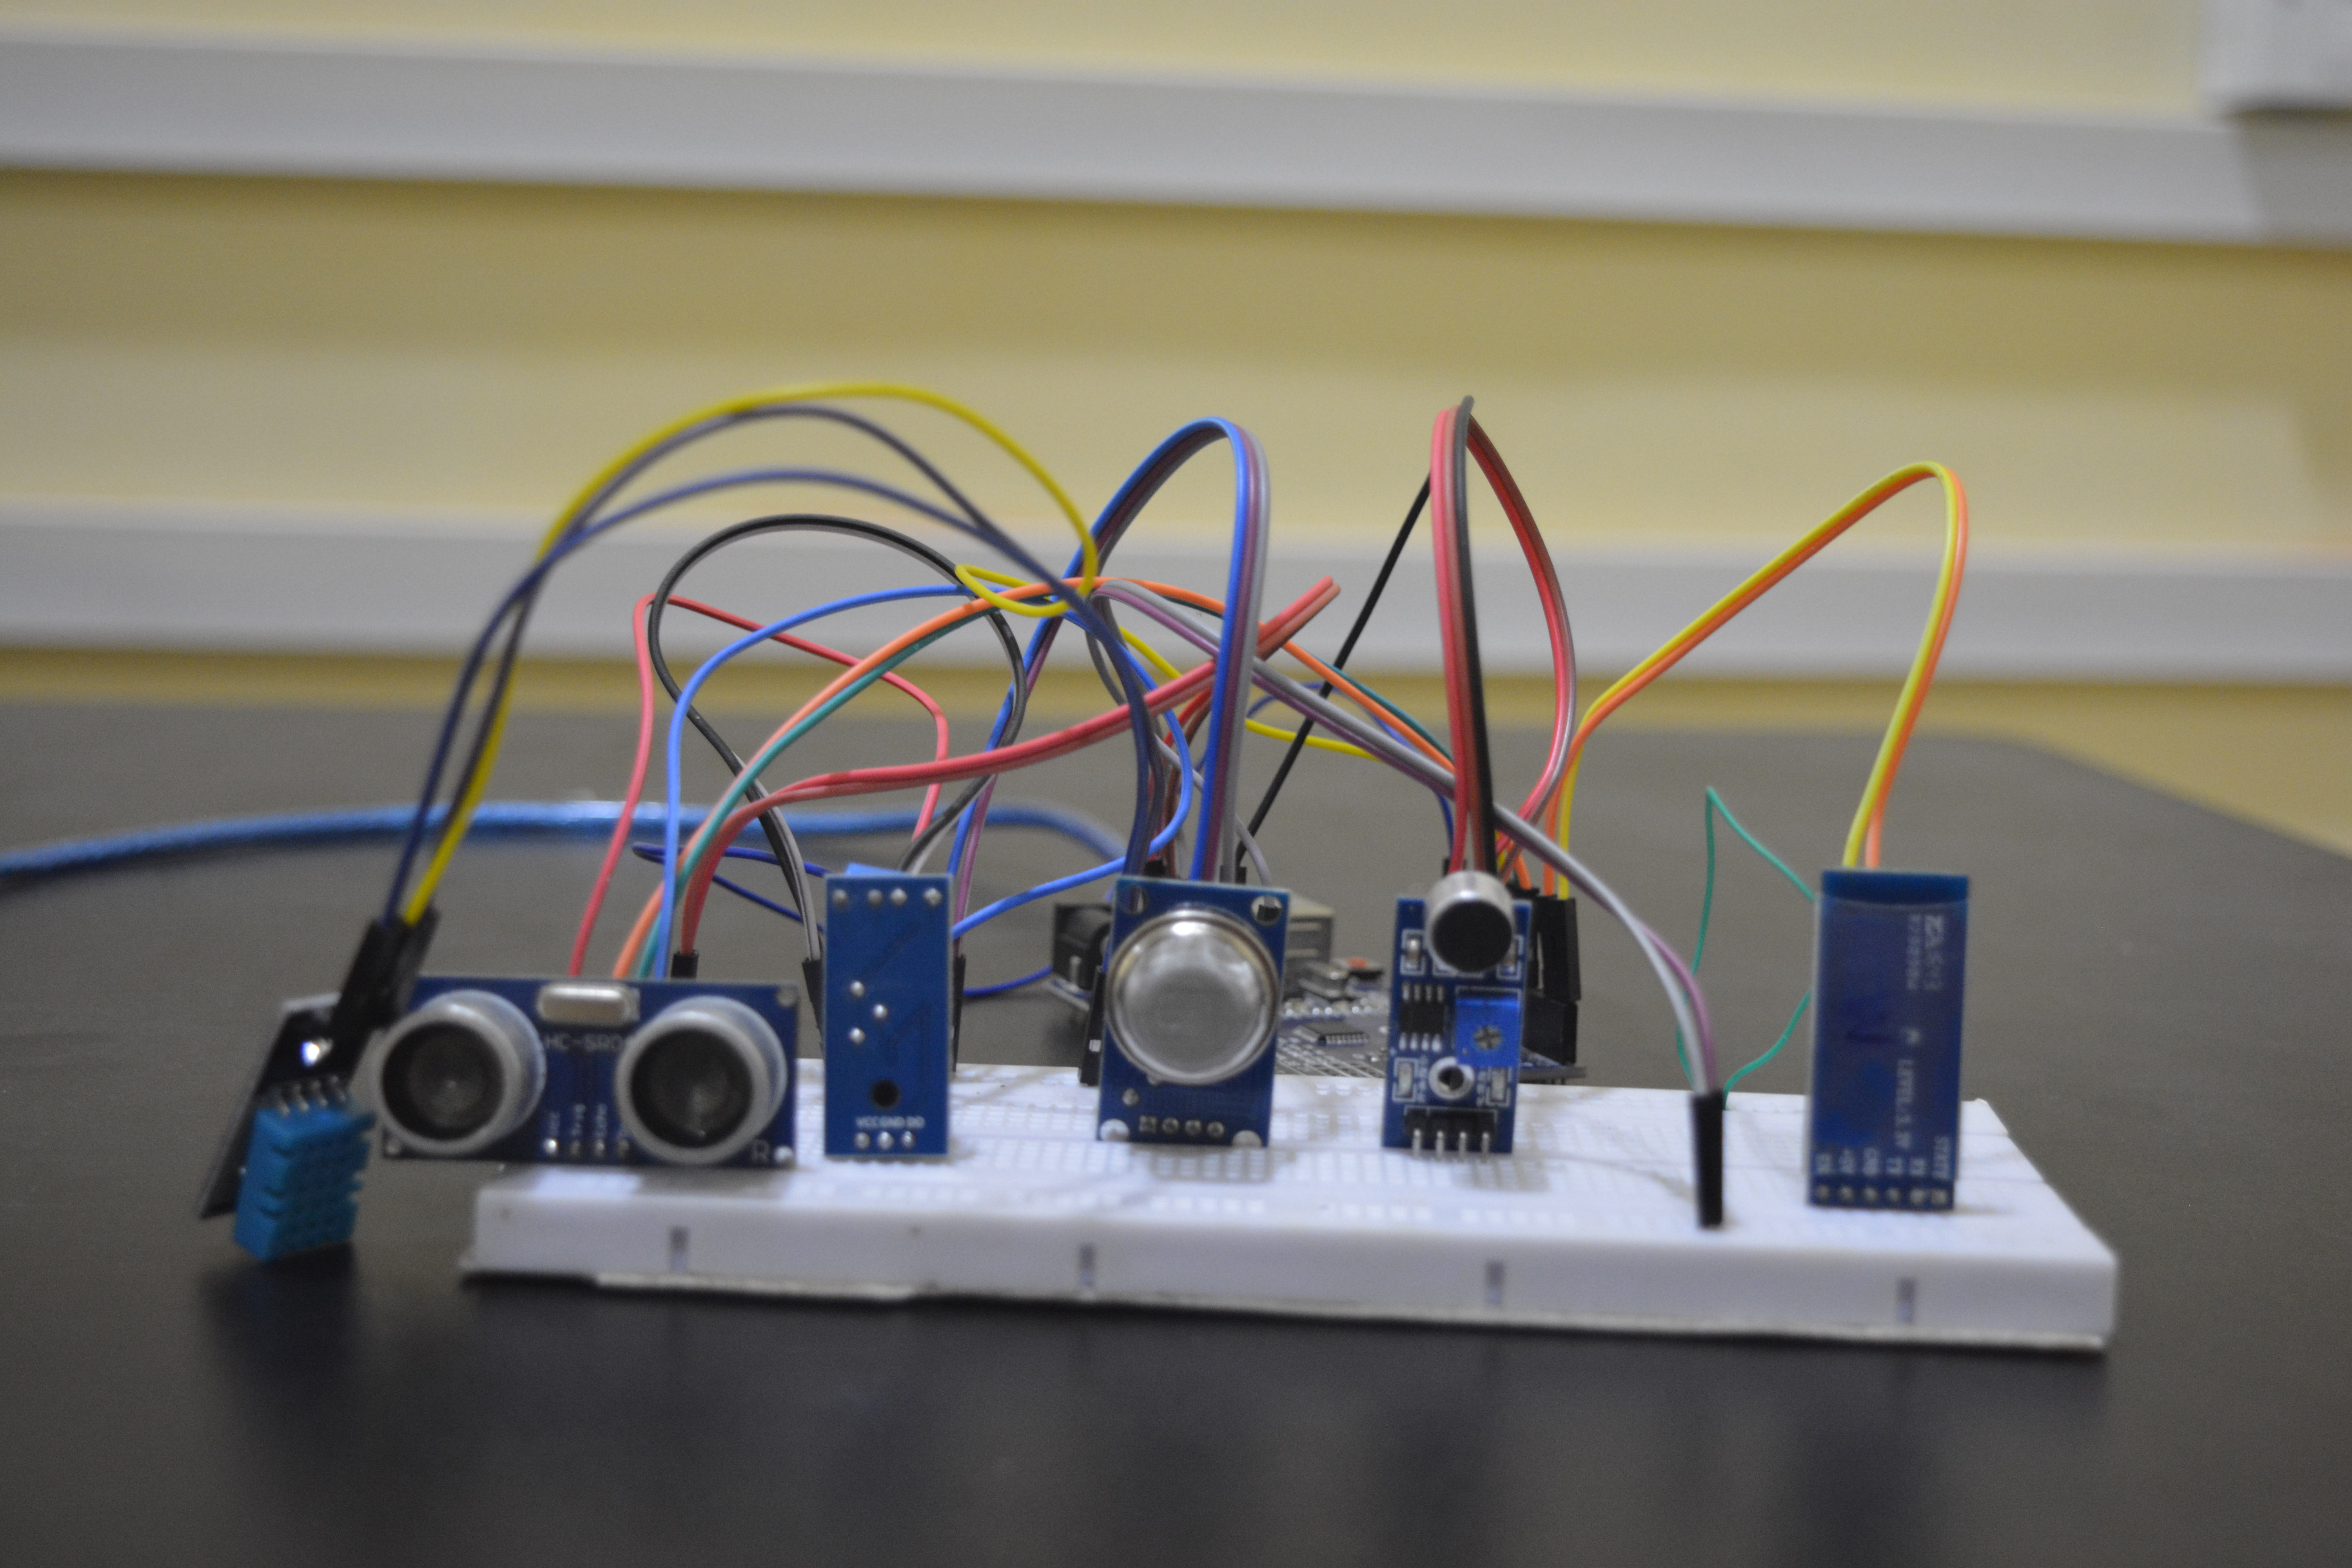
\includegraphics[width=4.0in]{master2.JPG}}
  \caption{ \textbf{}Master device to collect data from the sensors}
  \end{figure}
\end{frame}
\begin{frame}\frametitle{Slave  device}
  \begin{figure}
  \centerline{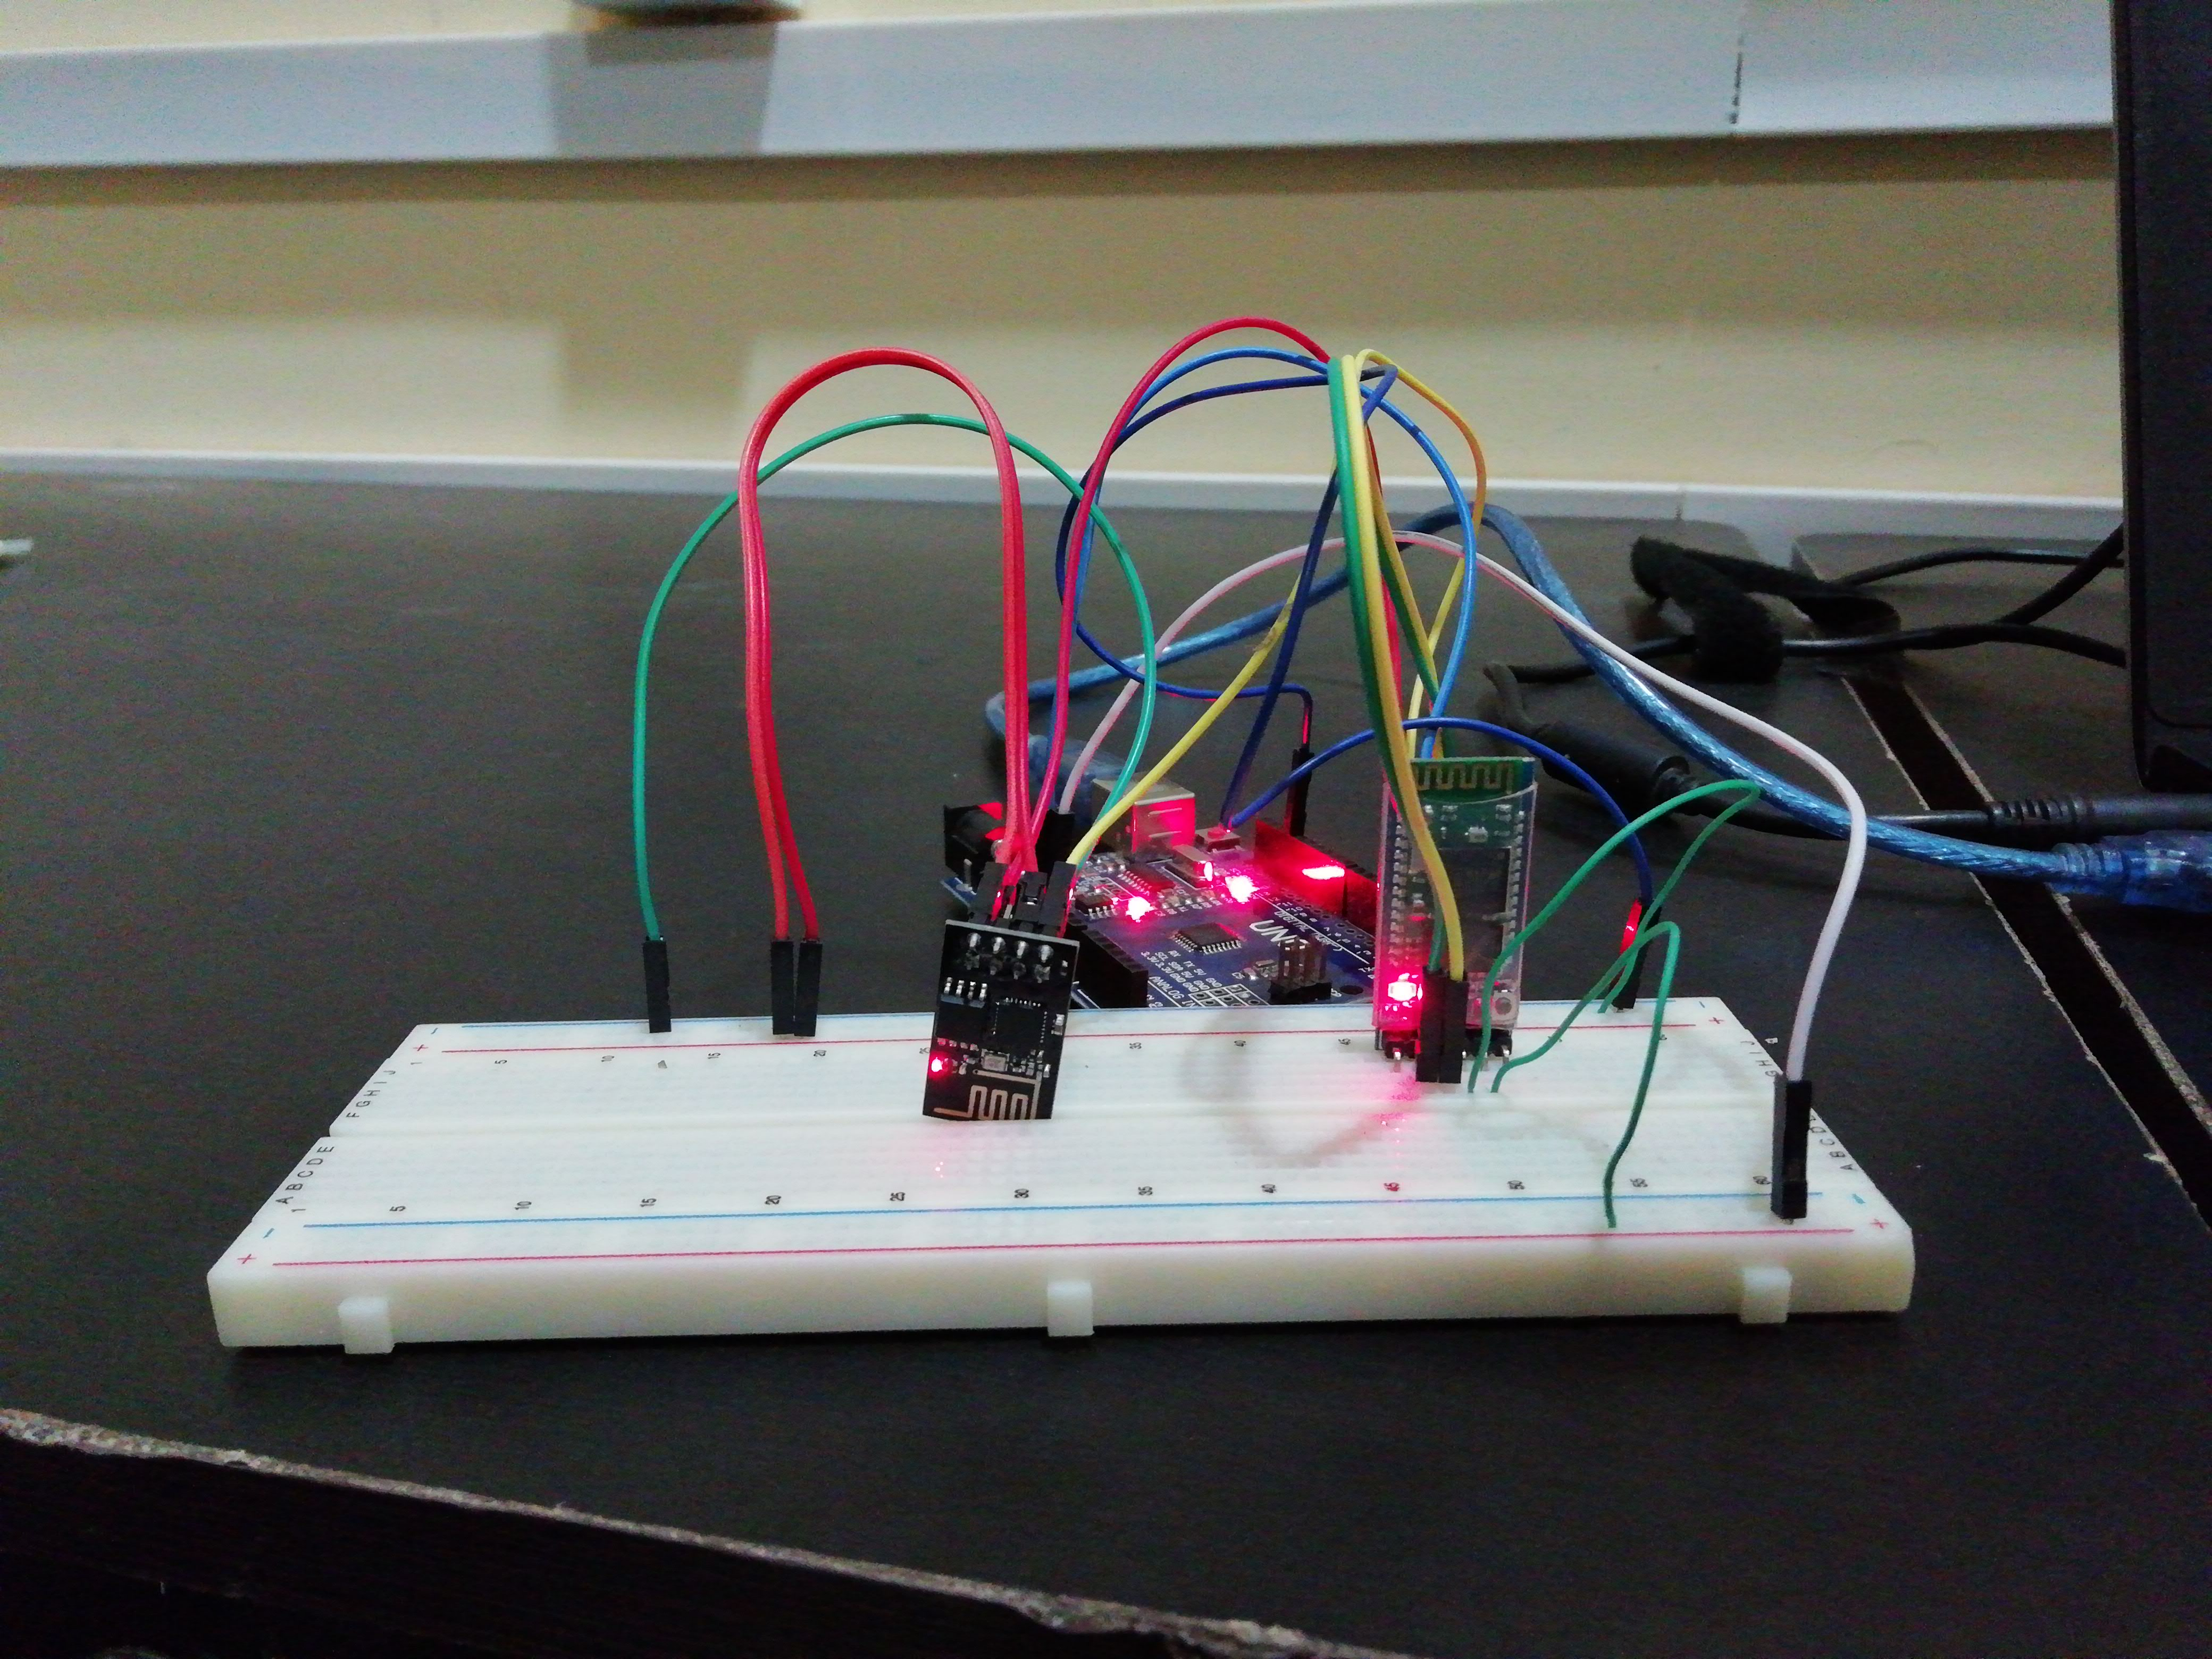
\includegraphics[width=4.0in]{sl}}
  \caption{ \textbf{}Slave device to transfer data to the cloud}
  \end{figure}
\end{frame}
\begin{frame}\frametitle{Communication between master and slave device amd data transmission to cloud }
\begin{itemize}
\item Bluetooth module is used to communicate between master and slave device.
\item A master Bluetooth module is connected to master device to send data to the slave device. 
\item A slave Bluetooth module is connected to slave device to receive data from the master device.
\item Bluetooth modules used serial port protocol for communication between two device.
\end{itemize}
\item Data transmission to cloud
\begin{itemize}
    \item ESP2866 WI-FI module is used to send sensor data into cloud
    \item We had used Think-Speak cloud to save our sensor data intocloud
\end{itemize}
\end{frame}

\begin{frame}\frametitle{Testing}
\begin{itemize}
\item We have tested few sensors on different environments.
\item We also used different set of sensors for different. requirements.  
\end{itemize}
\end{frame}
\begin{frame}
\begin{itemize}\frametitle{Results}
\item We have integrated five sensors on a single micro controller for effective reliability. 
\item We have established a wireless communication between two devices.
\item We have used different configuration of sensors for different environments.
\item The data collected is stored in a cloud storage for documentation.
\end{itemize} 
\end{frame}
\begin{frame}
\begin{itemize}
\item Data representation for ultrasonic sensor and sound sensor in cloud.
  \begin{figure}[H]
  \centerline{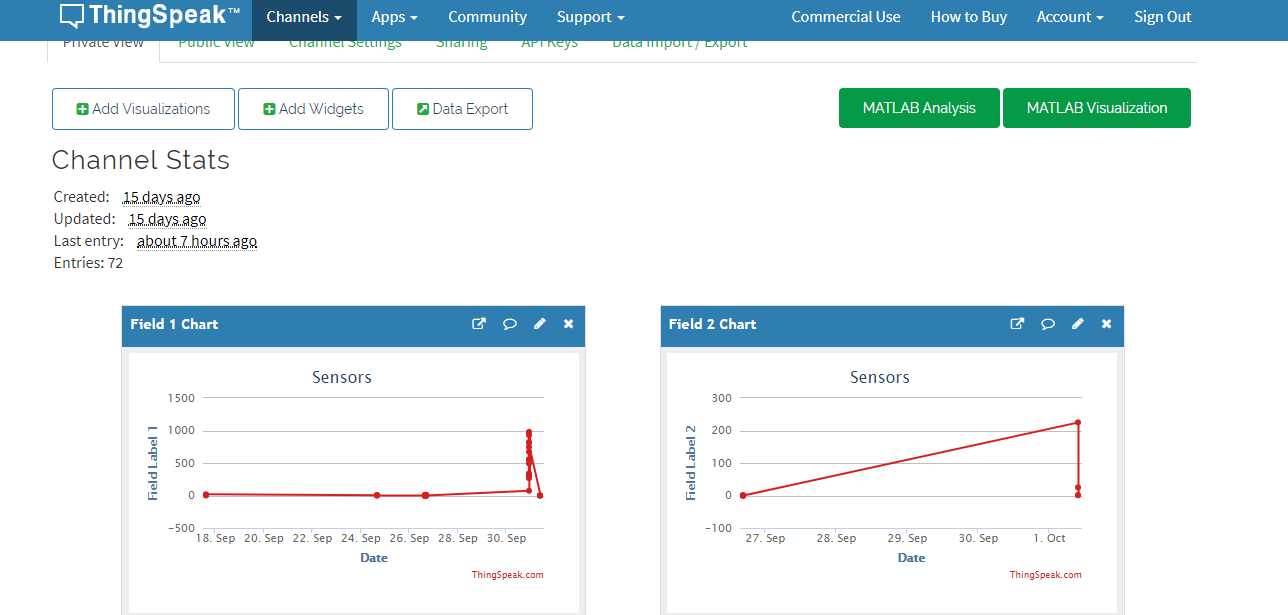
\includegraphics[width=4.0in]{01.JPG}}
  \caption{ \textbf{}Data representation in cloud for two sensors}
  \end{figure}
\end{itemize}
\end{frame}
\begin{frame}
\begin{itemize}
\item Data representation for multiple sensors in cloud.
  \begin{figure}
  \centerline{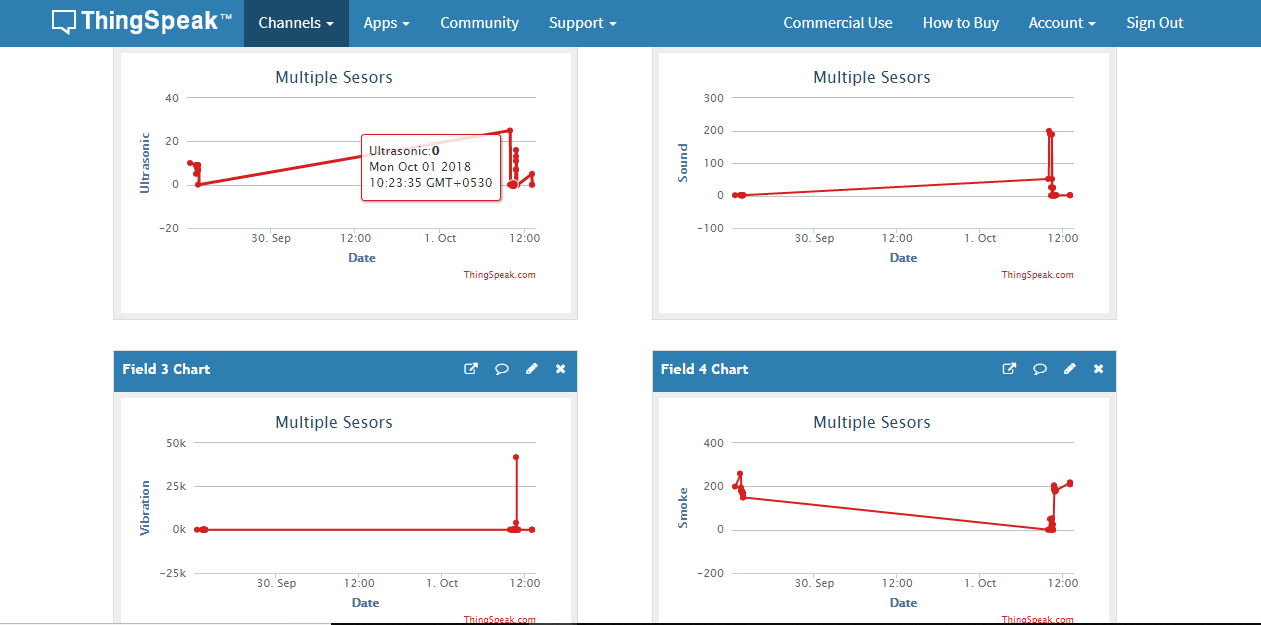
\includegraphics[width=4.0in]{22.JPG}}
  \caption{ \textbf{}Data representation in cloud for multiple sensors}
  \end{figure}
\end{itemize}
\end{frame}

\begin{frame}\frametitle{Conclusion}
\item 
\begin{itemize}
    
\end{itemize}
\begin{itemize}
\item Our main prospect of the project dealing with making an low cost IoT application which can become handy for the many industrial process and in the maintenance prospects .
\item 
Important factor which our objective results is in decreasing the employee engagement and automation of the security system which help companies to shape up economically.
\end{itemize}
\end{frame}
\begin{frame}\frametitle{Future Work}
Future work may comprise
\begin{itemize}
\item As a future work we will test our project in the industries.
\item The data stored in the cloud is sorted to set a threshold value for better health monitoring of industrial machines.
\Item 
\end{itemize}
\end{frame}
\begin{frame}[shrink=25]\frametitle{References}
\Item 1] Bank, Dirk. "A novel ultrasonic sensing system for autonomous mobile systems." IEEE Sensors Journal 2.6 (2002): 597-606
\Item 2] Bell, Charles. Beginning sensor networks with Arduino and Raspberry Pi. Apress, 2014
\item 3] Steiner, James P., and Greg Edward Sloan. "Ultrasonic sensing system." U.S. Patent Application No. 14/569,618
\item 4]  Beck, Maurice S. Process tomography: principles, techniques and applications. Butterworth-Heinemann, 2012
\item 5] Sobota, Jaroslav, et al. "Raspberry Pi and Arduino boards in control education." IFAC Proceedings Volumes 46.17 (2013): 7-12
\item 6] Maksimovic, Mirjana, et al. "Raspberry Pi as Internet of things hardware: performances and constraints." design issues 3 (2014).
\item 7] Mahowald, Peter H. "Method and apparatus for using a sound sensor to adjust the audio output for a device." U.S. Patent No. 8,306,235. 6 Nov. 2012.
\item 8] Cicolani, Jeff, and Jeff Cicolani. "Raspberry Pi and Arduino." Beginning Robotics with Raspberry Pi and Arduino: Using Python and OpenCV (2018): 129-185
\end{frame}

\begin{frame}\frametitle{}
\Huge
\begin{center}Thank You \end{center}
\end{frame}



\end{document}